\documentclass[10pt,conference,compsocconf]{IEEEtran}

\usepackage{hyperref}
\usepackage{graphicx}	% For figure environment
\usepackage{comment}
\usepackage{amssymb}
\usepackage{amsmath}
\usepackage{multirow}
\usepackage{tablefootnote}

\begin{document}
\title{Collaborative-Based Recommendation System}

\author{
  Farah Charab, Lorenzo Lazzara, Andrea Manzini\\
  \textit{EPFL, School of Computer and Communication Sciences}
}

\maketitle

\begin{abstract}
	In this work, we study the problem of recommending items to users using a collaborative-based filtering approach. In particular, we are only given access to users and their ratings, and we would like to recommend new movies by predicting the missing ratings. To this end, we implement 16 different models. A modified version of Singular Value Decomposition (SVD++) performs the best among these models. It achieves a score of $0.97671$ on Kaggle's validation set. In order to improve our predictions even further, we implement a ridge regression model that predicts ratings based on the predictions of 13 different models. We obtain a slight improvement over SVD++, increasing our accuracy score to $0.97368$ on Kaggle's validation set. Finally, we explore and implement some further models proposed by Koren ~\cite{koren2010factor}.
\end{abstract}
\begin{IEEEkeywords}
Baseline, Collaborative-Based Filtering, K-Nearest Neighbors (KNN), Ridge Regression, Matrix Factorization, Netflix Data, Singular Value Decomposition (SVD, SVD++), Recommendation.
\end{IEEEkeywords}
\section{Introduction}
Recommendation systems have became increasingly popular in recent years and have changed the way users interact with inanimate websites and applications. They are used in a variety of domains including (but not limited to) recommending movies, music, articles, search queries, and products/services in general. Recommendation systems can be broadly divided into three categories: collaborative-based systems, content-based systems, or a hybrid of both. Content-based systems examine the properties of the items and the user's preferences. On the other hand, collaborative-based filtering approaches are based on collecting and analyzing a large amount of information on users' behaviors, activities or preferences and predicting what users will like based on their similarity to other users. \\
In this work, we are given no access to any content information. Thus, we will stick to collaborative-based filtering systems. An important note to make is that in real life scenarios, one might be able to provide better recommendations if content data (name of movies, genre, actors/actress, etc..) or any additional features/statistics of user's activities (rating timestamps for example since users' preferences might vary over time) are available. \\
The remainder of this report is organized as follows: We first start by discussing some data statistics and exploration. We then discuss the various models we implemented, and the results we have obtained. We conclude the study with the model(s) we propose and some further thoughts.
\section{Data Exploration}
The training data consists of ratings provided by $10000$ users on a subset of $1000$ movies. The ratings are integer values that vary between $1$ and $5$, with $1$ being the lowest possible rating and $5$ being the highest. We extensively explored the data, but we will only discuss some of our findings.\\
Initially, we thought that among the many rating profiles, we might have two interesting extreme ones. In particular, we looked for users that strictly rated movies they hate, and those who strictly rated movies they loved. The reason behind this exploration was motivated by the idea that if we have many such users, then we might be able to extract additional features by labeling/learning whether a user might hate/like a movie. However, as shown in figure \ref{fig::users_means} , the ratings are concentrated around $3.8$. That is, on average users rate both movies they like or hate. In fact, there were no users who only gave ratings of $1$. Similarly, there were no users who only gave ratings of $5$. \\
\begin{figure}[h!]
    \caption{User Means Distribution}
    \centering
    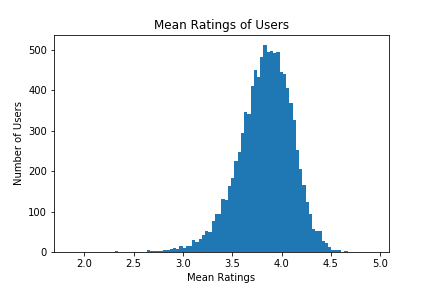
\includegraphics[width=0.8\columnwidth]{figure1.png}
    \label{fig::users_means}
\end{figure}
Furthermore, we look at different groups of users which we refer to as bloggers and new users. The bloggers are the top $5\%$ and the new users are the lowest $5\%$ of the users, where users are ordered by the number of their ratings. 
In particular, any user with more than $253$ rating is considered a blogger, and any user with at most $19$ ratings is considered a new user. An interesting behaviour is that there seem to be an almost increasing ``linear'' relationship between the ratings and their distribution, except for the following two regions: the region between the ratings $5$ and $4$ for the bloggers, and the region between the ratings $2$ and $3$ for the new users. This can base seen in figures \ref{fig::bloggers} \& \ref{fig::new_users}, respecitvely.
\begin{figure}[h!]
    \caption{New Users Ratings Distribution}
    \centering
    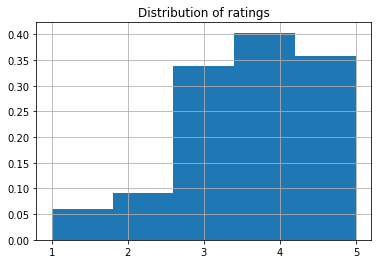
\includegraphics[width=0.4\textwidth]{figure2.png}
    \label{fig::new_users}
\end{figure}
\begin{figure}[h!]
    \caption{Bloggers Distribution}
    \centering
    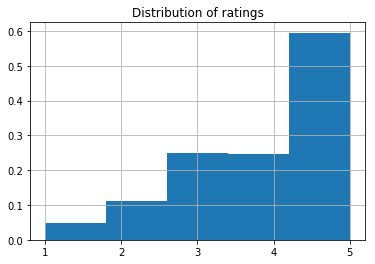
\includegraphics[width=0.4\textwidth]{figure3.png}
    \label{fig::bloggers}
\end{figure}
The data suggests that users tend to watch and thus rate movies they believe they will like. There might be several explanations for the gaps between ratings $2$ and $3$ for the new user. One possible explanation we considered is that new users don't treat consecutive points as equidistant, and hence they regard rating $2$ as too low for some movies. We thought of incorporating this into our models, by adjusting the ratings so that the distribution of ratings has an almost linear relationship with the ratings, however, we didn't have enough reason to justify such an assumption. Additionally, we were not able to explain the gap in the bloggers data, thus we decided to leave the data as is. \vspace{-5pt}
\section{Models}
Table \ref{table::summary} summarizes the RMSE results we obtained for all the models we included in the final blending, the weights assigned when blending the different models using ridge regression (see section \ref{section::blending}), and the running times of the various models when run on an Intel Core i7-6700HQ, 8Gb RAM . In what follows, we give a brief overview of the algorithms we implemented.
\begin{table}[h!]
  \centering
  \scalebox{0.8}{
  \begin{tabular}{|c||c|c|c|}
    \hline
    \# Method & RMSE & Computation Time (in minutes) & Weights \\ \hline \hline
    Baseline & $0.9974$ & $<1$& $-0.2272$ \\ \hline
    Global Mean &$1.1143$&$<1$ & $0.1677$ \\ \hline 
    Item Mean &$1.0285$ &$<1$& $-0.0914$\\ \hline
    Item Median &$1.0992$ &$<1$& $-0.0154$ \\  \hline
    User Mean &$1.0915$&$<1$& $-0.2250$\\ \hline
    User Median &$1.1476$&$<1$& $0.0239$ \\ \hline
    KNN Item&0.9852&$5$&$0.2175$\\ \hline
    KNN User &0.9893&$50$&$0.3583$\\ \hline
    Matrix Factorization (ALS)&0.9847&$13$& $-0.0066$\\ \hline
    Matrix Factorization (SGD) &0.9895&$13$& $0.0111$\\ \hline
    Slope One &0.9982&$<1$& $-0.2586$\\ \hline
    SVD &0.9805&$3$&$-0.8426$\\ \hline
    SVD++ &0.9777& $140$& $1.8864$\\ \hline
    Blending &0.97368&$<1$\tablefootnote{This is only the overhead running time we get when blending the different models. That is, assuming we have predictions of the various models already computed.}& - \\ \hline
  \end{tabular}}
  \caption{Summary on the Models Implemented \tablefootnote{The RMSE of all the models is calculated using $6 \%$ of the training data set, except that of the blending model. The RMSE of the blending model is obtained from Kaggle's validation set.}}
  \label{table::summary}
\end{table}
\vspace{-5pt}
\subsection{Global Mean \& Median}
The simplest model is to compute the mean or the median value of the non-zero ratings in the training set, and return this value as the prediction. This gives a baseline score from which we can compare further models. 
\subsection{Users Mean \& Median}
Another simple model is to compute the mean or median of the ratings given by a user. The mean of the ratings of user $n$ can be computed as follows.
\begin{equation}
\hat{x}_n := \frac{1}{|\Omega_{n:}|} \sum_{m \in \Omega_{n:}}{} x_{nm}
\end{equation}
where $\Omega_{n}$ is the set of movies rated by the $n^{th}$ user. The median can be computed in a similar fashion.
\subsection{Items Mean \& Median}
Another simple model is to compute the mean or median of the ratings given to a movie. The mean of the ratings given to a movie $m$ can be computed as follows. 
\begin{equation}
\hat{x}_m:= \frac{1}{|\Omega_{:m}|} \sum_{n \in \Omega_{:m}}{} x_{nm}
\end{equation}
where $\Omega_{m}$  is the set of users who rated the $m^{th}$ movie. The median can be computed in a similar fashion.
\subsection{Baseline}
The baseline predictions are the base on which most of the complex models are built on. It provides biases for each user and each item and combines them together with the global mean to make predictions. From this point onwards, another algorithm can add deviations from the baseline model using a different criteria, with the advantage of working with unbiased ratings. Normally, the biases would be extrapolated using ridge regression over the ratings. However, we use a model specified by Koren ~\cite{koren2010factor}, based on ALS, which is lighter than ridge regression but gives similar results. This algorithm is implemented in the Python Surprise library ~\cite{Surprise}.
\subsection{KNN User Based}
Before the Netflix Prize, it was the most common model in recommendation systems ~\cite{koren2010factor}. This model builds a similarity matrix over the users and utilizes it to find the $k$ most similar users to a given one. For the similarity matrix, we use a baseline pearson similarity metric since this metric accounts for the biases of the ratings per user/movie. This criteria is computationally heavier than the other metrics (mean squared difference, pearson, cosine) because it makes some effort to deal with the biases. This algorithm is implemented in the Python Surprise library ~\cite{Surprise}.
\subsection{KNN Item Based}
As the previous model, this builds a baseline pearson similarity matrix, but over the items and uses it to find the $k$ most similar items to a given one. It is preferred to the user based KNN for the following reasons.
\begin{itemize}
\item Usually items are much less numerous than users, so the the algorithm is computationally less expensive.
\item Adding a new user to the system doesn't involve the re-computation of all the weights, so it is easier to manage.
\item Recommendations can be explained, improving the overall users' satisfaction. When the system suggests a movie, it can indicate the movie (or the movies) watched by the user in the past that brought the system to that particular recommendation. In a user based KNN, this kind of explanation is impossible due to privacy restrictions and is not useful anyway.
\end{itemize}
This algorithm implemented in the Python Surprise library ~\cite{Surprise}.
\subsection{Matrix Factorization SGD}
Given $D$ movies and $N$ users, we define  $X \in {\mathbb{R}}^{N \times D}$ to be the matrix containing all ratings. We aim to find two matrices $W \in {\mathbb{R}}^{K \times D}$ and  $Z \in {\mathbb{R}}^{K \times N}$, such that $X \approx Z^{T}W$. In order to find these matrices we minimize the following quantity.
\begin{equation}\label{eqn::SGD}
\frac{1}{2} \sum_{(d, n) \in |\Omega}{} [x_{nd} -(\mathbf{Z^TW})_{nd}]^2 + \frac{\lambda _w}{2} \Vert \mathbf{W} \Vert ^2 + \frac{\lambda _z}{2} \Vert \mathbf{Z} \Vert ^2 
\end{equation}
where $K$ is the number of latent features, and $\lambda_{z}$, $\lambda_{w}$ are scalar constants that weigh the regularization terms. \\
The stochastic gradient descent is a stochastic approximation of the gradient descent optimization.The gradient of the objective function is computed by chosing a random element of the summation.
\subsection{Matrix Factorization ALS}
ALS is one of the main alternatives to the SGD to solve (\ref{eqn::SGD}). It is a two-step iterative algorithm. In every iteration, it first fixes $Z$ and solves for $W$, and then it fixes $W$ and solves for $Z$. Fixing one matrix at a time, the problem is reduced to a linear regression and a simple least squares technique can be used. 
\subsection{SVD (Matrix Factorization)}
Despite the name, which became common during the Netflix Prize, this model does not utilize a Singular Value Decomposition. Instead it is a matrix factorization with SGD as before, but it includes the learning of biases in the least square problem. This allows to take into account all those inclinations of users and items which are not easily accounted for by the matrix features (for example famous/unknown movies and enthusiastic/strict users). This algorithm is implemented in the Python Surprise library ~\cite{Surprise}.
\subsection{SVD++ (Matrix Factorization With Implicit Ratings)}
This model is an extension of SVD, but it takes into account implicit ratings as proposed by Bell \& Koren ~\cite{koren2008factorization, koren2010factor}. In a real life scenario, especially in streaming services, lots of information can be considered as implicit ratings such as number of views, continuity and frequency of watching and so on. With our reduced dataset, we can only consider the fact that a user decided to rate a movie as an implicit rating, no matter what the rating is. We are not sure about what meaning to give to this factor, that's why the system automatically learns it for us. The SVD++ algorithm is very powerful, but it is also slow and difficult to tune. That is why we suggest not to use it unless one has more meaningful implicit factors. This algorithm is implemented in the Python Surprise library ~\cite{Surprise}.
\subsection{Slope One}
The prediction $\hat{r}_{ui}$ is set as follows.
\begin{equation}
\hat{r}_{ui} = \mu _u + \frac{1}{|R_{i}(u)|} \sum_{j \in R_{i}(u)}{}  dev(i, j)
\end{equation}
where $R_{i}(u)$ is the set of relevant items. The set of relevant items is the set of items $j$ rated by user $u$ that have at least one common user with item $i$, and $dev(i,j)$ is defined as the average difference between the ratings of $i$ and those of $j$. That is,
\begin{equation}
dev(i, j) = \frac{1}{|U_{ij}|} \sum_{u \in U_{ij}}{} (r_{ui} - r_{uj})
\end{equation}
This algorithm is implemented in the Python Surprise library ~\cite{Surprise}.
\subsection{Blending}\label{section::blending}
As explained in ~\cite{koren2009bellkor}, the smallest RMSE can be achieved using a combination of different methods instead of an individual predictor. We decided to proceed in the same direction in order to obtain our final model. We approach blending as a linear regression problem. We use the Python module $sklearn.linear\_model$ in order to find the weights for a linear combination of the models (referred to as linear blend in ~\cite{koren2009bellkor}). We choose the ridge regression as an estimator in order to avoid overfitting and assigning meaningless weights to the different models. Using a simple linear regression estimator without regularization gave us huge weights (positive and negative) for the global mean and global median
\footnote{ After the introduction of the regularizer,  the weight assigned to the global median was zero, so we decided to exclude it from the models. That's why it does not appear in any table or in the code.} models which however compensate each other, but did not give useful information on the real influence of these models. \\
For the blending, we split the data in $93.3\% $ and $6.7\%$ (equivalent to $15$ folds in a cross validation). Then we use the $93.3\%$ to train the models and the $6.7\% $ to train the ridge regression. 
To compute the final ratings, we compute the ratings for each model, and then combine them using the weights found by ridge regression.
\subsection{Surprise Library Customization}
The Surprise library was customized for performance enhancements. In particular we introduced the following functionalities:
\begin{itemize}
\item Shuffling of datapoints during the SGD of SVD and SVD++: In the original code, the order of the examined datapoints was the same at each iteration of the algorithms, depriving the Gradient Descent from the ``stochastic'' property.
\item Scaling of learning rates at each iteration of the gradient descent in SVD and SVD++: This can help finding the minimum, especially in SVD++ where the high number of parameters makes the minimization very sensitive. We chose to scale by a factor of $0.9$, as proposed by Koren et al ~\cite{koren2009bellkor}.
\item Computational speed improvement in SVD++: We compute user fixed information (number of ratings, items rated) once at the beginning of the algorithm, instead of calculating it inside the for loop over all the ratings in the train set (as done by the library). This modification allows to almost double the speed of the algorithm, while maintaining the same results.
\item Initialization of baseline in SVD++: We initialize the baseline parameters with the ones computed by the BaselineOnly model instead of using an array of zeros. This initialization can bring some improvement in this complex model, where wrong biases can easily make the SGD inefficient.
\item Optimization of baseline pearson similarity computation: Before estimating the baseline for the similarity matrix, we check if they were already computed. This fix can help especially when doing a grid search over the parameters
\end{itemize}
Two other completely custom algorithms have been implemented in the Surprise framework: FactorizedNeighborhood and WeightedNeighborhood. They were proposed by Koren et al. during the Netflix Prize \cite{koren2008factorization, koren2010factor}. We didn't include these models in the blending because unfortunately we couldn't obtain a satisfying RMSE when using them. This may be caused by an error in the implementation or by the fact that it is very difficult to find the right parameters to feed them with. Thus, more tests should be performed before proposing a push into the original library. In the next two sections, we provide a brief explanation of the models and some details on their implementations.
\subsection{Weighted Neighborhood}
This model was proposed by Bell and Koren during the Netflix Prize \cite{koren2008factorization, koren2010factor}. It avoids using a specific similarity measure which could affect the ratings in an unnatural way. On the contrary, it lets the algorithm learn the weights with SGD and introduces new biases, learnt during the iterations, which respond to the new scale of the weights. The function that estimates the prediction is the following.
\begin{align}
\hat{r}_{ui} = \mu + b_{u} + b_{i} &+ \nonumber\\
&|R^{k}(i;u)|^{-\frac{1}{2}} \sum_{j \in R^{k}(i;u) }(r_{uj}-b_{uj})w_{ij} + c_{ij}  
\end{align}
where $\mu$ is the global mean, $b_{uj}$ are the baseline estimations computed with the BaselineOnly algorithm, $b_{u}$, $b_{i}$, $w_{ij}$, $c_{ij}$ are learnt with simple SGD over the regularized quadratic error (see \cite{koren2008factorization,koren2010factor} for more details), $w_{ij}$ corresponds to the weights assigned to the neighbors ratings and $c_{ij}$ takes care of the implicit ratings.
\subsection{Factorized Neighborhood}
This model is an extension of the Weighted Neighborhood which also includes the matrix factorization estimation \cite{koren2008factorization}. It somehow corresponds to a blending, but it is done directly during the learning, so it should be more powerful. The parameters are learnt using the linear SGD proposed in the paper, which tries to minimize the regularized quadratic error. The estimations are given by
\begin{align}
\hat{r}_{ui} &= \mu + b_{u} + b_{i} + q_{i}^{T}(p_{u} + |R(u)|^{-\frac{1}{2}} \sum_{j \in R(u)}y_{j}) \nonumber \\
&+ |R^{k}(i;u)|^{-\frac{1}{2}} \sum_{j \in R^{k}(i;u)} (r_{uj}-b_{uj})w_{ij} + c_{ij} 
\end{align}
Since this algorithm is computationally very heavy, efforts were made in order to optimize the code. The most important step in this direction was achieved using the Cython compiler. \footnotetext{Cython is an optimizing static compiler for both the Python programming language and the extended Cython programming language (based on Pyrex). The Cython language is very close to the Python language, but Cython additionally supports calling C functions and declaring C types on variables and class attributes.  This allows the compiler to generate very efficient C code from Cython code(http://cython.org/).} In order to make the compiler produce an efficient C code, we tried to observe (as much as possible) some rules while writing the functions critic for the computation time:
\begin{itemize}
\item For the variables we used Cython fixed types instead of Python dynamic types.
\item Indexing of numpy arrays were done without slicing, inside for loops over the single elements.
\item We use memoization when possible, avoiding to compute the same quantities more than once.
\item Bounds check and wrap around of arrays were disabled.
\end{itemize}
\section{Conclusions}
In this paper, we showed that combining different methods can improve RMSE of the final prediction. While individual models score an RMSE of at least $0.977$, blending achieves an RMSE of around $0.973$. The blending improves the score since models can compensate for each other. \\
We achieved $0.97349$ as final score on Kaggle's validation set using the blending technique we described. Further improvements could be possibly attained by either combining more methods, using a different blending technique, or even using the same models but with different parameters.The models are very sensitive to the variation of the parameters, so running a grid search with a very dense refinement for each parameter can improve the model. However the drawback is the high computational time of such a process. 
\bibliographystyle{plain}
\bibliography{references}
\end{document}
